\section{Related work}
\label{sec:related_work}
\begin{figure}[t]
    \centering
    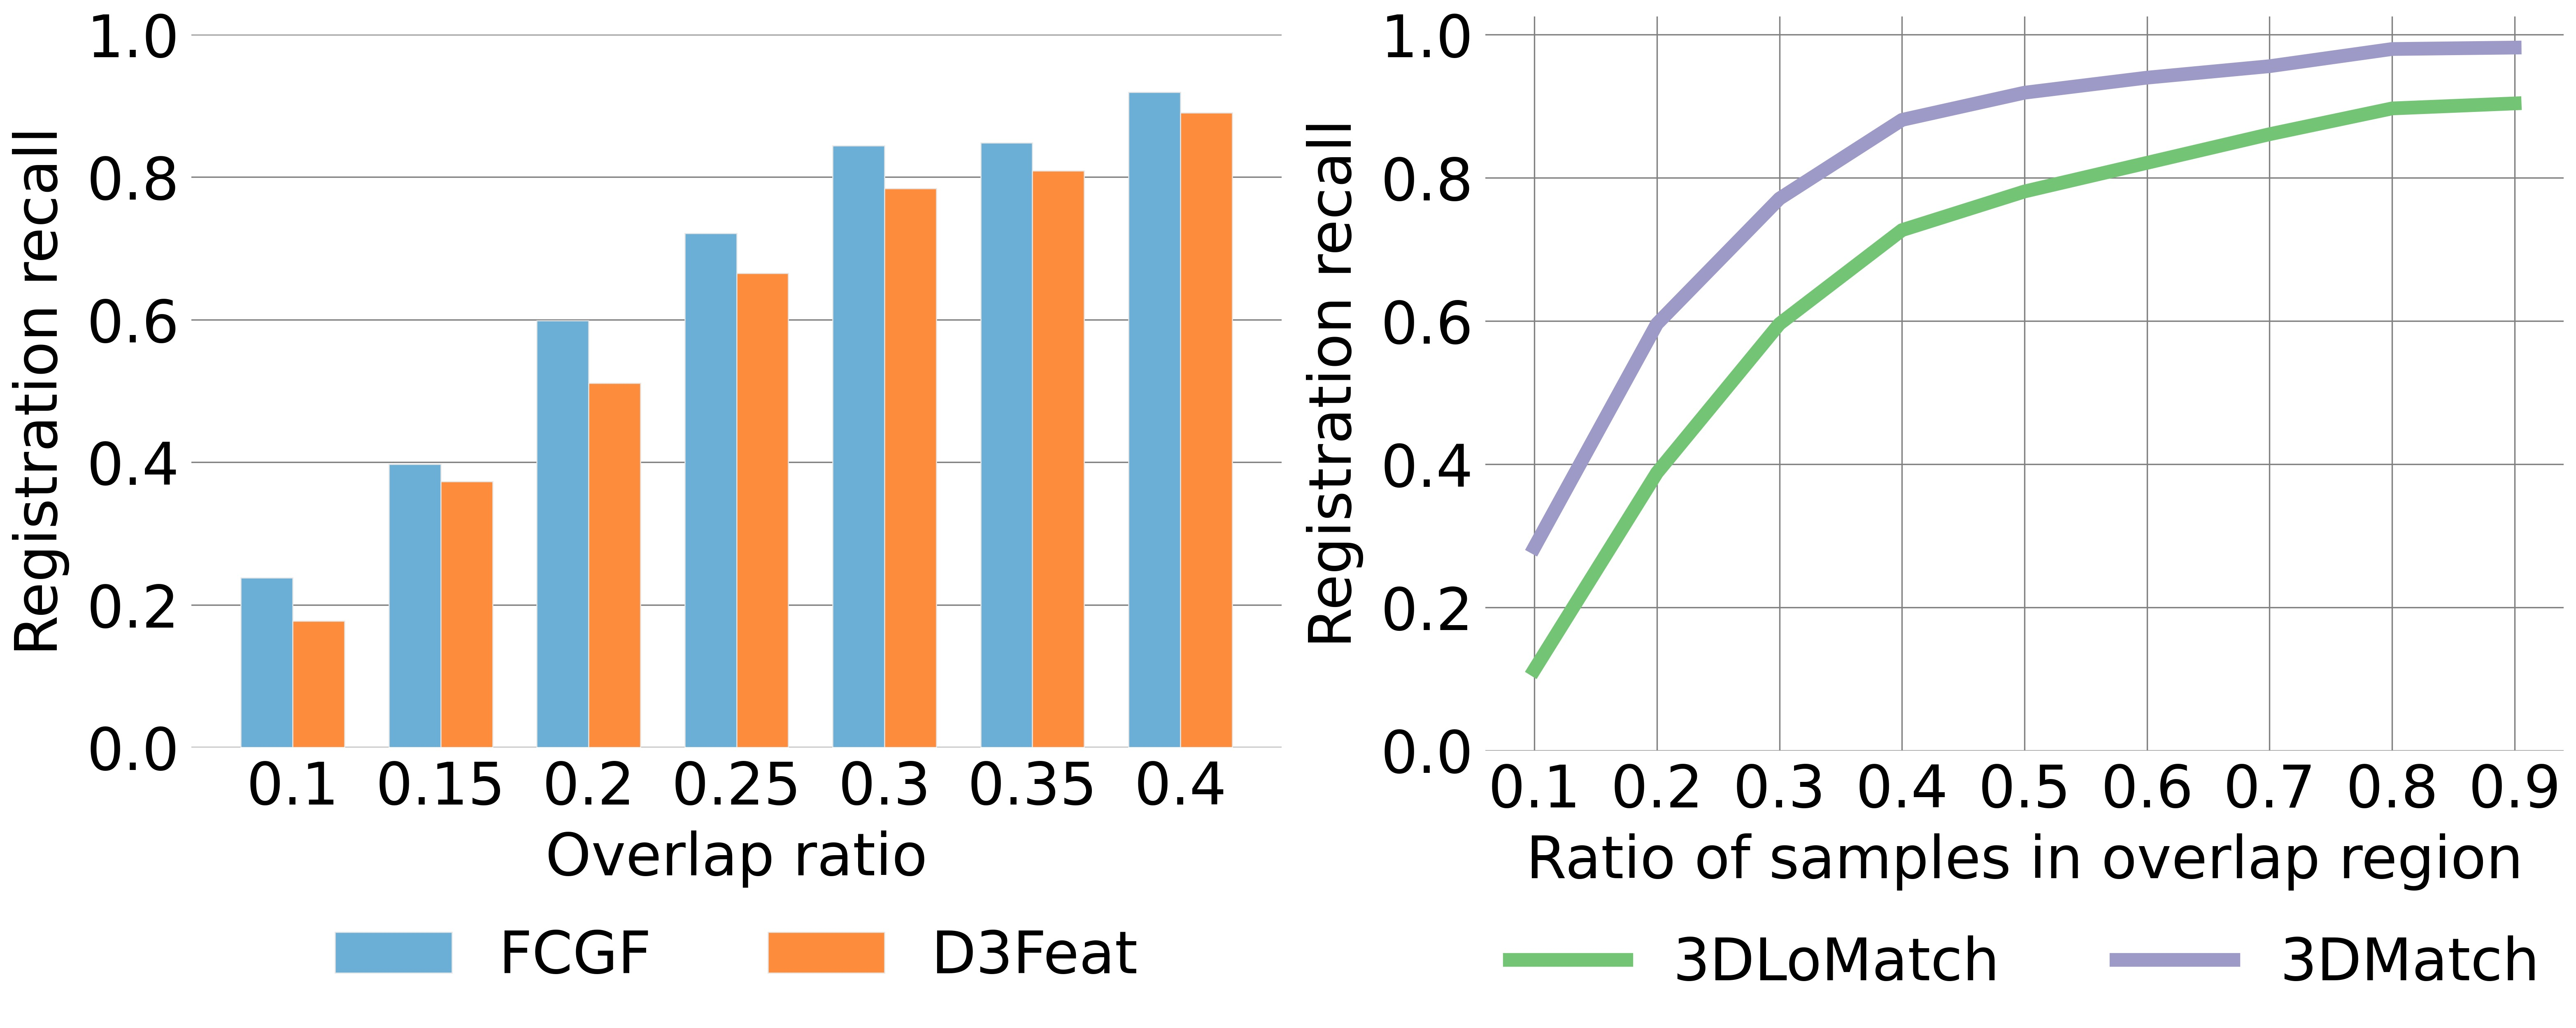
\includegraphics[width=0.8\columnwidth]{figures/images/motivation.jpg}
    \caption{Registration with SoTA methods deteriorates rapidly for pairs with $<$30\% overlap (\textit{left}). By increasing the fraction of points sampled in the overlap region, many failures can be avoided as shown here for FCGF~\cite{Choy2019FCGF} (\textit{right}).} 
    \label{fig:motivation}
    
\end{figure}
\begin{figure}[t]
    \centering
    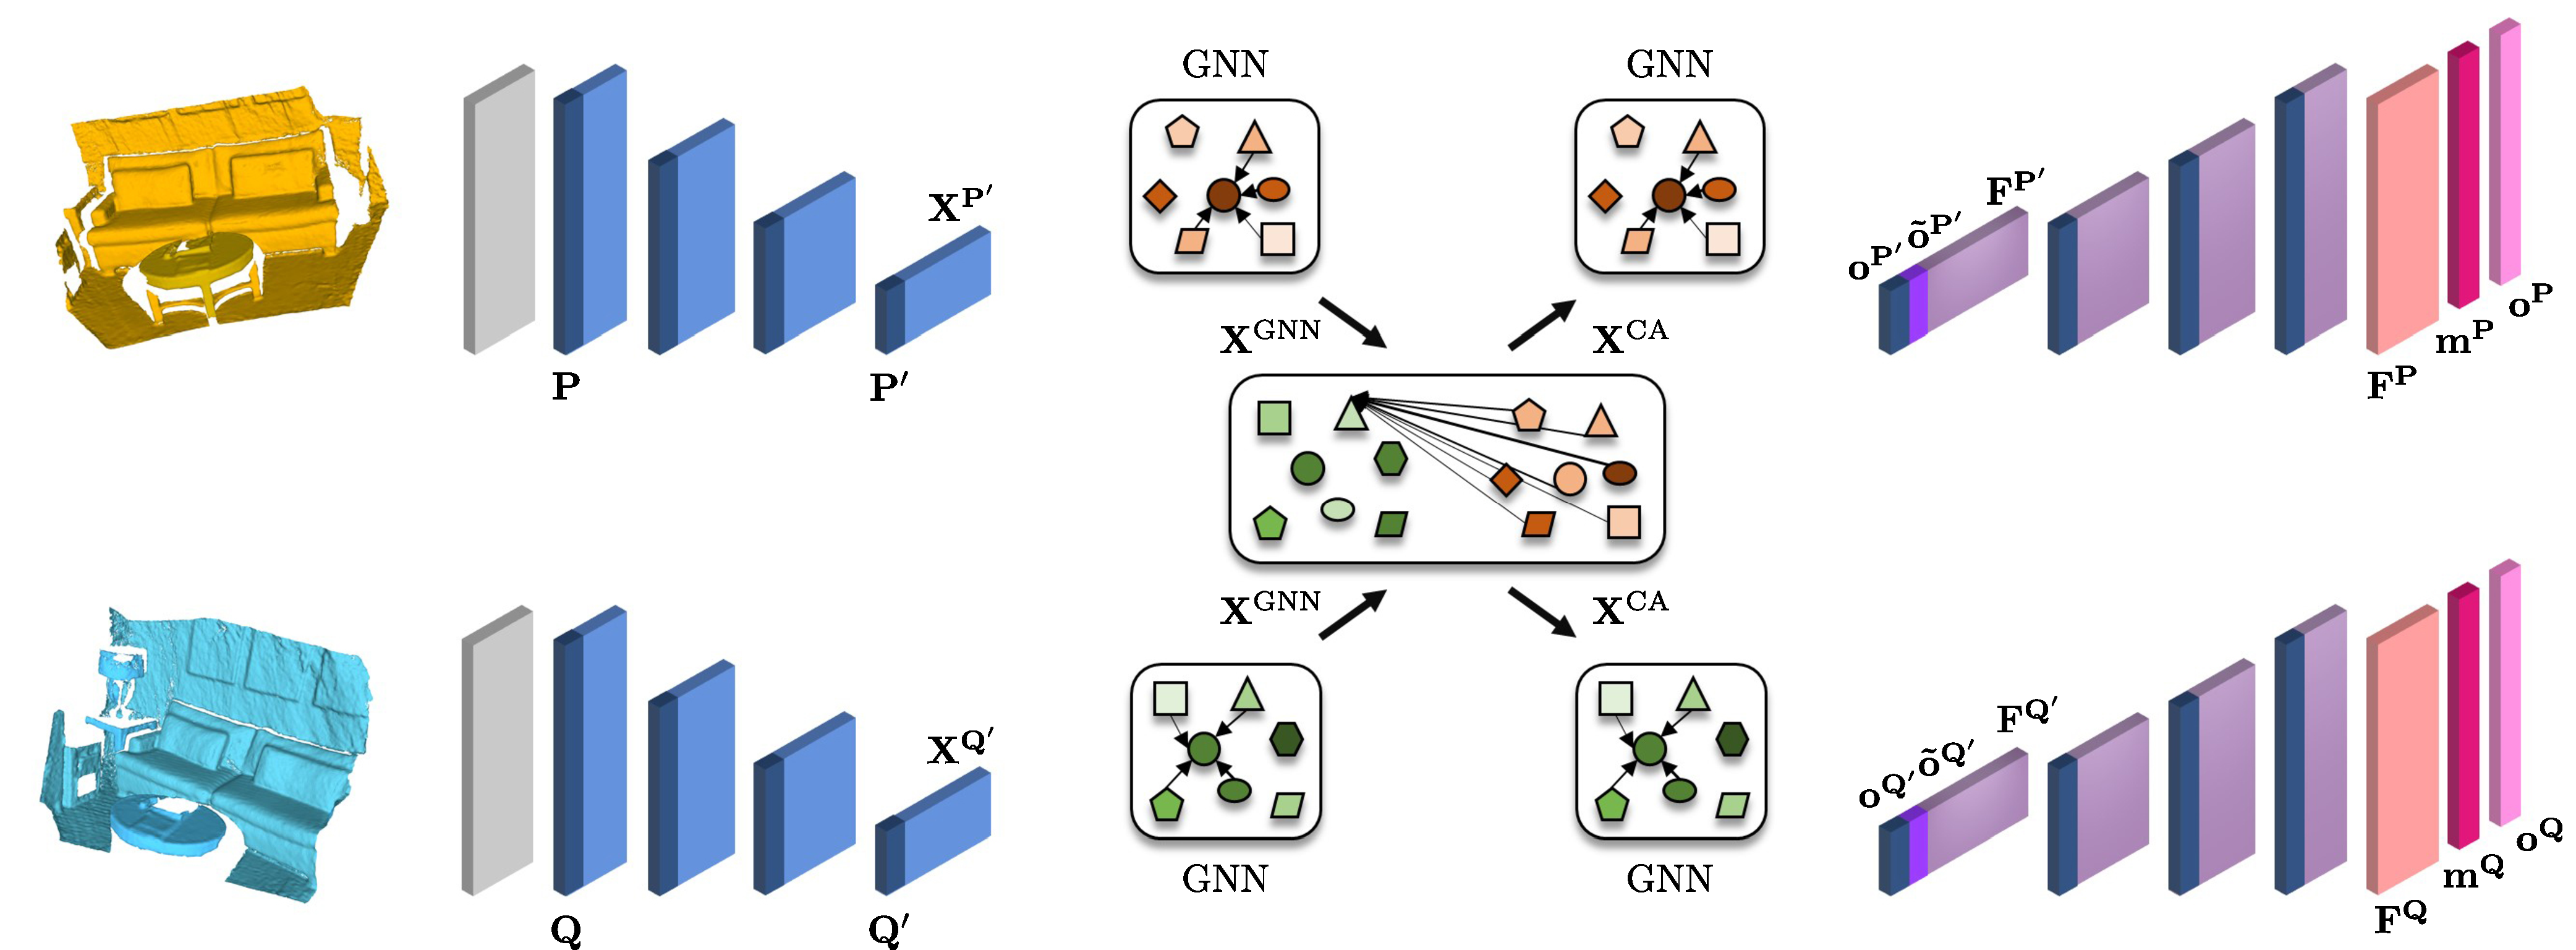
\includegraphics[width=0.9\textwidth]{figures/images/network_architecture.pdf}
    \caption{Network architecture of \acro. \textcolor{gray}{Voxel-gridded} point clouds $\mathbf{P}$ and $\mathbf{Q}$ are fed to the encoder, which extracts the superpoints $\mathbf{P}'$ and $\mathbf{Q}'$ and their latent features $\mathbf{X}^{\mathbf{P}'}$, $\mathbf{X}^{\mathbf{Q}'}$. The overlap-attention module updates the features with co-contextual information in a series of self- (GNN) and cross-attention (CA) blocks, and projects them to overlap  $\mathbf{o}^{\mathbf{P}'}$, $\mathbf{o}^{\mathbf{Q}'}$ and cross-overlap $\tilde{\mathbf{o}}^{\mathbf{P}'}$, $\tilde{\mathbf{o}}^{\mathbf{Q}'}$ scores. Finally, the decoder transforms the conditioned features and overlap scores to per-point feature descriptors $\mathbf{F}^\mathbf{P}$, $\mathbf{F}^\mathbf{Q}$, overlap scores $\mathbf{o}^\mathbf{P}$, $\mathbf{o}^\mathbf{Q}$, and matchability scores $\mathbf{m}^\mathbf{P}$, $\mathbf{m}^\mathbf{Q}$.}
    \label{fig:network_arch}
    
\end{figure}

We start this related-work section by reviewing the individual components of the traditional point cloud registration pipelines, before proceeding to newer, end-to-end point-cloud registration algorithms. Finally, we briefly cover recent advances in using contextual information to guide and robustify feature extraction and matching.

% \cameraready{Point cloud registration usually follows local feature extraction, interest point sampling, and RANSAC or Kabsch algorithm for pose estimation. Since point cloud registration requires context from both scans, we conclude this section with contextual information.}

\paragraph{Local 3D feature descriptors} 
Early local descriptors for point clouds~\cite{johnson1999, rusu2008PFH, rusu2009FPFH, tombari2010SHOT, tombari2010USC} aimed to characterise the local geometry by using hand-crafted features. While often lacking robustness against clutter and occlusions, they have long been a default choice for  downstream tasks because they naturally generalise across datasets~\cite{guo2014performanceEvaluation}. In the last years, learned 3D feature descriptors have taken 
over and now routinely outperform their hand-crafted counterparts.

The pioneering 3DMatch method~\cite{zeng20163dmatch} is based on a Siamese 3D CNN that extracts local feature descriptors from a signed distance function embedding.
Others~\cite{khoury2017CGF, gojcic2018learned} first extract hand-crafted features, then map them to a compact representation using multi-layer perceptrons. PPFNet~\cite{deng2018ppfnet}, and its self-supervised version PPF-FoldNet~\cite{Deng2018PPFFoldNetUL}, combine point pair features with a PointNet~\cite{qi2017pointnet} architecture to extract descriptors that are aware of the global context. To alleviate artefacts caused by noise and voxelisation,~\cite{gojcic20193DSmoothNet} proposed to use a smoothed density voxel grid as input to a 3D CNN. These early works achieved strong performance, but still operate on individual local patches, which greatly increases the computational cost and limits the receptive field to a predefined size.

Fully convolutional architectures~\cite{long2015fully} that enable dense feature computation over the whole input in a single forward pass~\cite{detone2018superpoint, dusmanu2019d2Net, revaud2019r2d2} have been adopted to design faster 3D feature descriptors. Building on sparse convolutions~\cite{choy2019Minkowski}, FCGF~\cite{Choy2019FCGF} achieves
a performance similar to the best patch-based descriptors~\cite{gojcic20193DSmoothNet}, while being orders of magnitude faster. D3Feat~\cite{bai2020d3feat} complements
a fully convolutional feature descriptor with an salient point detector. 


\paragraph{Interest point sampling} 
The classic principle to sample salient rather than random  points
has also found its way into learned 2D~\cite{detone2018superpoint, dusmanu2019d2Net,revaud2019r2d2, wiles2020d2d} and 3D~\cite{yew20183dfeat, bai2020d3feat,lu2020rskdd} local feature extraction.
All these methods implicitly assume that the saliency of a point fully determines its utility for downstream tasks. Here, we take a step back and argue that, while saliency is desirable for an interest point, it is not sufficient on its own. Indeed, in order to contribute to registration a point should not only be salient, but must also lie in the region where the two point clouds overlap---an essential property that, surprisingly, has largely been neglected thus far.


\paragraph{Deep point-cloud registration} 
Instead of combining learned feature descriptors with some
off-the-shelf robust optimization at inference time, a parallel stream of work aims to embed the differentiable pose estimation into the learning pipeline. PointNetLK~\cite{aoki2019pointnetlk} combines a PointNet-based global feature descriptor~\cite{qi2017pointnet} with a Lucas/Kanade-like optimization algorithm~\cite{lucas1981LK} and estimates the relative transformation in an iterative fashion.
DCP~\cite{wang2019dcp} use a DGCNN network~\cite{wang2019dynamic} to extract local features and computes soft correspondences before using the Kabsch algorithm to estimate the transformation parameters. To relax the need for strict one-to-one correspondence, DCP was later extended to PRNet~\cite{wang2019prnet}, which includes a \textit{keypoint} detection step and allows for partial correspondence. Instead of simply using soft correspondences, ~\cite{yew2020rpm} %
update the similarity matrix with a differentiable Sinkhorn layer~\cite{sinkhorn1964relationship}. Similar to other methods, the weighted Kabsch algorithm\cite{4767965} is used to estimate the transformation parameters. Finally, ~\cite{gojcic2020learning,choy2020deep,pais20203dregnet}
complement a learned feature descriptor with an outlier filtering network, which infers the correspondence weights for later use in the weighted Kabsch algorithm. 



\paragraph{Contextual information} In the traditional pipeline, feature extraction is done independently per point cloud. Information %
is only communicated when computing pairwise similarities, although aggregating contextual information
at an earlier stage could provide additional cues to robustify the descriptors and guide the matching step.

In 2D feature learning, D2D-Net~\cite{wiles2020d2d} use an attention mechanism in the bottleneck of an encoder-decoder scheme to aggregate the contextual information, which is later used to condition the output of the decoder on the second image.
SuperGlue~\cite{sarlin2020superglue} infuses the contextual information into the learned descriptors with a whole series of self- and cross-attention layers, built upon the message-passing GNN~\cite{kipf2016semi}. 
Early information mixing was previously also explored in the field of deep point cloud registration, where~\cite{wang2019dcp, wang2019prnet} use a transformer module to extract task-specific 3D features that are reinforced with contextual information.

